%# -*- coding: utf-8-unix -*-

\chapter{相关技术}
\label{chap:related}

\section{基于内容推荐}

基于内容的推荐系统的特点是根据物品内容与用户偏好的契合度为用户进行推荐。系统首先需要通过文档、描述说明等资料对用户历史记录中的物品进行分析,建立物品档案;并基于物品的特征为用户建立偏好档案。为了能够直观、简单地为用户提供推荐,物品档案与用户偏好档案通常具有相同结构的模型。基于内容推荐算法首先将用户偏好和物品进行匹配。根据匹配度,我们可以得知用户对该物品的偏好程度。在假定用户档案可以精确反应用户偏好的前提下,可以根据用户档案为用户进行信息甄别与筛选,对解决信息超载问题有极大的帮助。

\subsection{基于内容推荐算法的系统架构}
基于内容的推荐系统需要对物品和用户档案使用合适的方法进行分析,还需要衡量用户偏好和物品相似度的策略。系统可以细分为三个关键组件,分别是内容分析、档案学习以及物品过滤。

在内容分析组件处理之前,物品通常是非结构化的。一般需要对物品进行预处理以提取结构相关信息。该组件的主要任务就是通过特征提取将物品从源信息空间迁移到目标空间,将物品的内容表示成适当的格式,以供在后两个组件中使用。第二个组件是档案学习,它对表示用户偏好的数据进行收集、归纳以建立用户档案。通常,可以通过统计学方法对数据进行收集,通过机器学习的方法对档案进行归纳,归纳的过程就是从用户偏好的物品和不喜欢的物品中,推导出用户的用户的兴趣模型。第三个组件是物品过滤,利用用户偏好档案与物品的相似度为用户推荐新物品。根据相似度衡量方式,计算结果包括离散型相似度以及连续型相似度。
将候选物品列表根据相似度进行排序,就可以得到推荐列表。

\begin{figure}
 \centering
 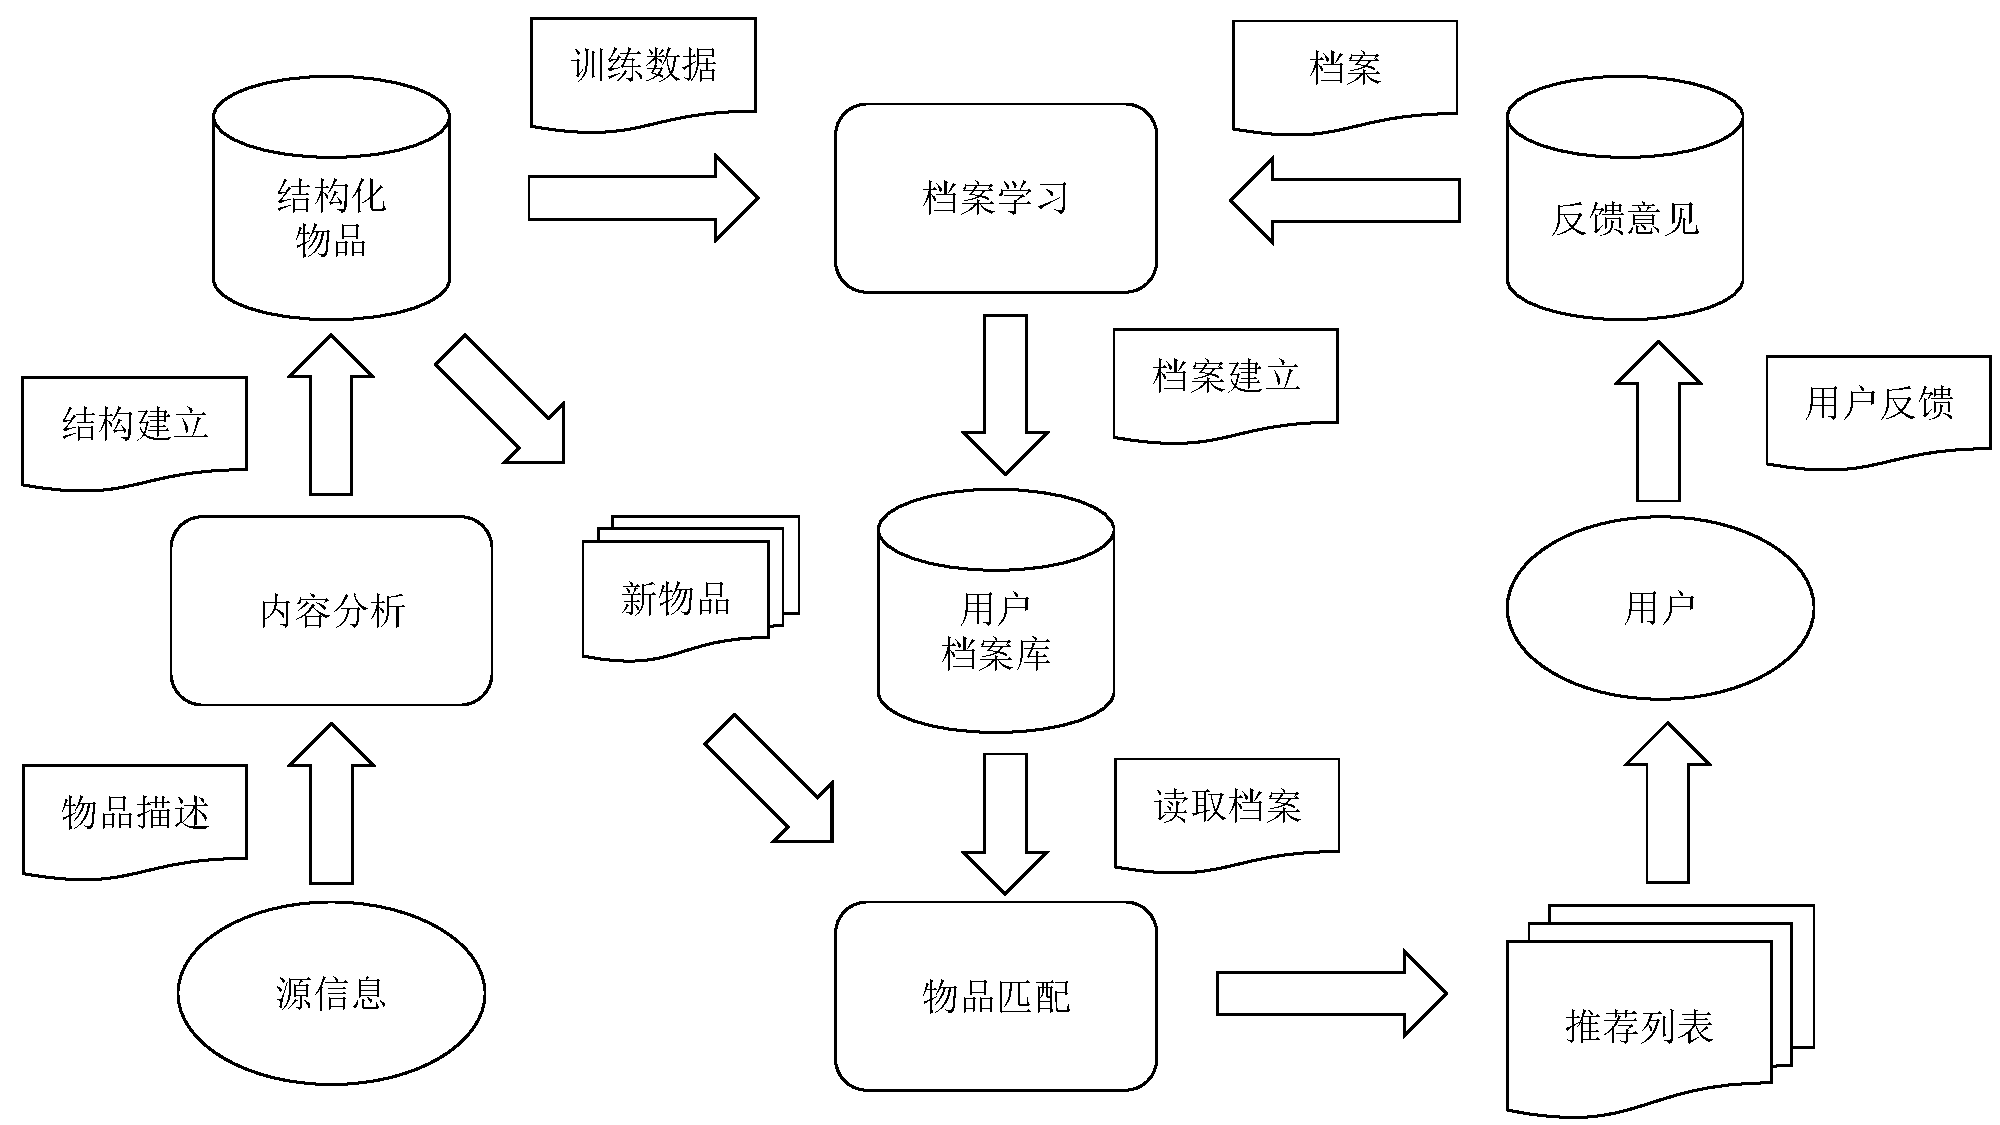
\includegraphics[width=0.75\linewidth]{02/1_cbr_arch.pdf}
 \bicaption[fig:cbr_arch]{推荐架构}{基于内容推荐算法的系统架构}{Fig}{Architecture of Content-based Recommender System}
\end{figure}

图\ref{fig:cbr_arch}展示了基于内容推荐算法的系统总体架构。其中椭圆形模块代表源数据,包括物品、用户信息;圆角矩形代表关键组件;圆柱形模块代表处理后的数据;箭头方向代表流程及数据流向。在内容分析组件中,通常会借用信息检索系统中的技术,为源信息中的物品提取特征,生成物品描述以及物品的结构化内容,并将其进行存储。

\subsection{基于内容推荐算法的推荐流程}

为了对用户档案进行创建及更新,需要存储用户对物品的反馈,这些反馈用于档案学习阶段。通常,用户反馈根据用户是否偏好该物品分为两种类型,分别是正反馈以及负反馈。根据反馈的获取方式,分为显式反馈和隐式反馈。其中,显式反馈由用户对物品的主动评价获得;而隐式反馈通过对用户行为的分析获得。显式反馈可以表明用户对物品的偏好程度以及相关性。总体上,显示反馈有三种表达方式。喜欢/反感 —— 用户使用二元评分机制将物品分为相关与不相关两类;打分 —— 使用离散的数值来表示对物品的评判。通常,将不同的喜好程度映射到不同的评分数值;文字评论 —— 依据用户对物品的评论来确定用户对物品的偏好。但需要自然语言处理的技术来判断评论是正面还是负面。

为了向用户提供推荐物品,需要为用户$u_a$定义训练集$TR_a$,对于显式反馈而言,$TR_a$的形式可以是物品-评分集合。档案学习组件通过有监督学习的算法生成预测模型,即用户偏好档案;并将档案存储在档案仓库中,供物品过滤组件使用。对于每一个结构化的物品,物品过滤组件会预测用户是否对该物品有偏好。将用户最可能偏好的$K$个物品生成一份推荐列表展示给用户。此外,用户的偏好可能会随时间改变。因此,系统还需维护用户的实时信息,如用户对推荐列表中物品的评价,产生新的训练集。用于档案学习组件对用户偏好的自动更新。



\section{主题模型}



\section{隐语义模型参数推导}